\chapter{Funcionamento do Sistema}

O sistema Love Letter é uma aplicação web multiplayer que permite aos usuários jogar o jogo de cartas Love Letter em tempo real através de seus navegadores. O funcionamento do sistema pode ser compreendido através de diferentes perspectivas: o fluxo de interação do usuário, a arquitetura técnica, e os mecanismos de sincronização em tempo real.

\section{Fluxo de Interação do Usuário}

\subsection{Autenticação e Gerenciamento de Conta}
O usuário inicia sua experiência criando uma conta ou fazendo login no sistema. O processo de autenticação utiliza tokens JWT para manter a sessão do usuário de forma segura. Após a autenticação, o usuário tem acesso ao dashboard principal, onde pode gerenciar seu perfil, visualizar salas disponíveis ou criar novas salas de jogo.

\subsection{Criação e Entrada em Salas}
O usuário pode criar uma nova sala de jogo, definindo um nome e opcionalmente uma senha para acesso restrito. Alternativamente, pode visualizar todas as salas disponíveis e entrar em uma delas. O sistema suporta até seis jogadores por sala, e cada sala possui um host (criador) que tem permissões especiais, como a capacidade de deletar a sala.

\subsection{Início da Partida}
Uma vez na sala, os jogadores aguardam o início da partida. O host pode iniciar o jogo quando houver pelo menos dois jogadores presentes. O sistema automaticamente distribui as cartas iniciais e determina a ordem de jogo, iniciando com o primeiro jogador, conforme ilustrado na Figura~\ref{fig:start-game-flow}.

\begin{figure}[h]
    \centering
    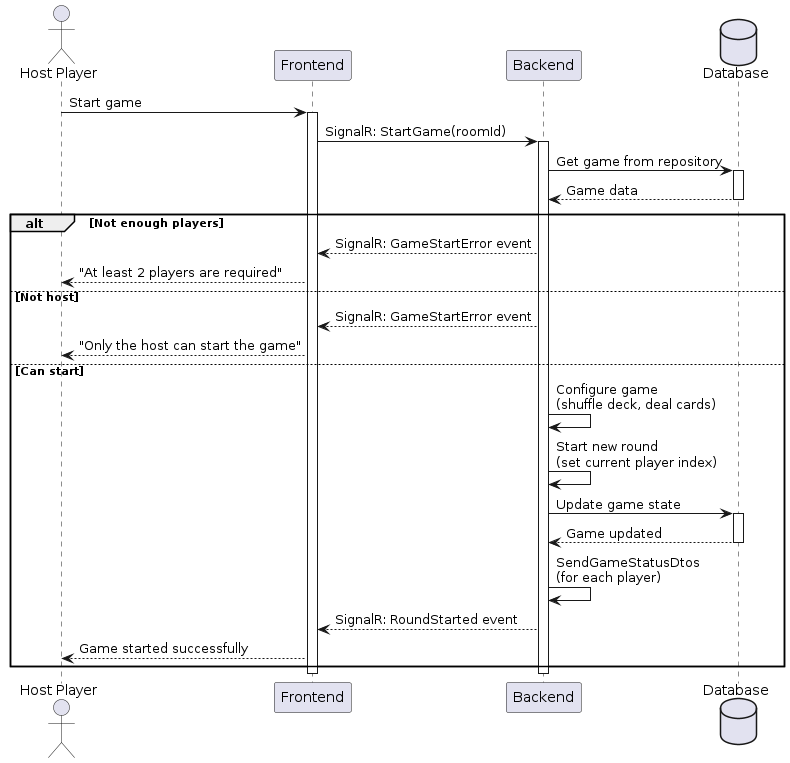
\includegraphics[width=0.8\textwidth]{diagrams/StartGame.png}
    \caption{Fluxo de início do jogo. Fonte: os autores}
    \label{fig:start-game-flow}
\end{figure}

A Figura~\ref{fig:start-game-flow} ilustra o processo de início do jogo. O host solicita o início da partida através da interface, o que dispara uma mensagem SignalR para o servidor. O sistema então valida se há jogadores suficientes (mínimo de 2) e se o solicitante é realmente o host da sala. Se todas as validações passarem, o sistema configura o jogo embaralhando o baralho, distribuindo as cartas iniciais e definindo o primeiro jogador. O estado do jogo é atualizado no banco de dados e todos os jogadores são notificados do início da rodada.

\section{Mecanismos de Jogo}

\subsection{Ciclo de Turno}
O jogo segue um ciclo de turnos bem definido:

\begin{enumerate}
    \item \textbf{Compra de Carta}: O jogador da vez compra uma carta do baralho, adicionando-a à sua mão
    \item \textbf{Jogada de Carta}: O jogador escolhe uma das duas cartas em sua mão para jogar, executando seu efeito específico
    \item \textbf{Resolução de Efeitos}: O sistema processa o efeito da carta jogada, que pode incluir eliminação de jogadores, proteção, troca de cartas, entre outros
    \item \textbf{Avanço de Turno}: O turno passa para o próximo jogador ativo
\end{enumerate}

O diagrama da Figura~\ref{fig:game-turn-flow} ilustra o fluxo geral dessas etapas durante um turno.

\begin{figure}[h]
    \centering
    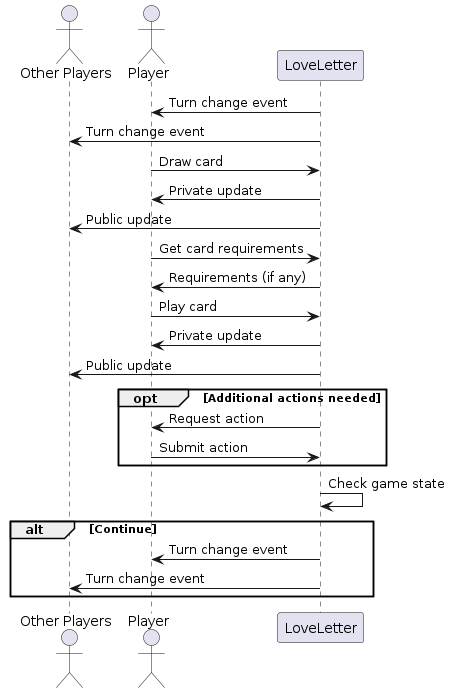
\includegraphics[width=0.4\textwidth]{diagrams/GameTurnFlow.png}
    \caption{Fluxo geral de um turno no jogo. Fonte: os autores}
    \label{fig:game-turn-flow}
\end{figure}

A Figura~\ref{fig:advance-turn-flow} ilustra o processo de verificação de finalização tanto de rodadas quanto do jogo completo. Após cada jogada, o sistema verifica se a rodada terminou (por eliminação de jogadores ou esgotamento do baralho). Se a rodada terminou, o sistema determina os vencedores e concede pontos bônus quando aplicável. Em seguida, verifica se o jogo completo terminou (quando um jogador atinge a pontuação necessária). Se o jogo não terminou, uma nova rodada é iniciada com a distribuição de novas cartas. Caso contrário, o turno simplesmente avança para o próximo jogador ativo.

\begin{figure}[h]
    \centering
    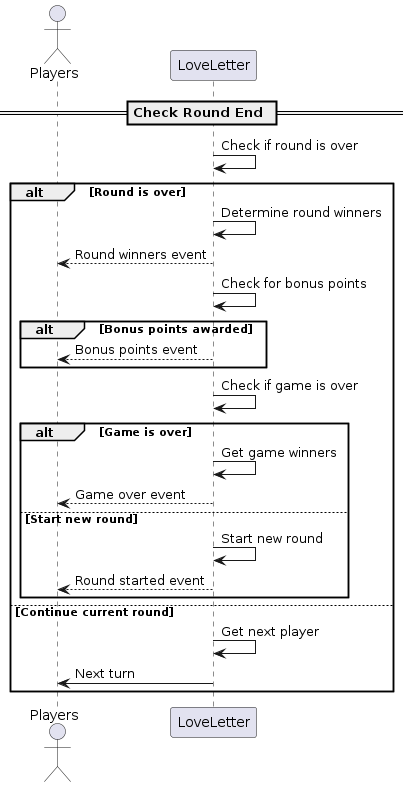
\includegraphics[width=0.35\textwidth]{diagrams/AdvanceTurnFlow.png}
    \caption{Fluxo de avanço de turno e verificação de finalização. Fonte: os autores}
    \label{fig:advance-turn-flow}
\end{figure}

\subsection{Sistema de Cartas}
O jogo utiliza 10 tipos diferentes de cartas, cada uma com valores e efeitos únicos, conforme ilustrado nas Figuras~\ref{fig:spy-card-play} a~\ref{fig:princess-card-play}:

\begin{itemize}
    \item \textbf{Espião (0)}: Concede ponto bônus se mantido até o final da rodada
    \item \textbf{Guarda (1)}: Permite adivinhar a carta de outro jogador
    \item \textbf{Padre (2)}: Permite olhar a carta de outro jogador
    \item \textbf{Barão (3)}: Compara cartas com outro jogador
    \item \textbf{Criada (4)}: Protege o jogador até seu próximo turno
    \item \textbf{Príncipe (5)}: Força outro jogador a descartar e comprar nova carta
    \item \textbf{Chanceler (6)}: Permite comprar duas cartas e escolher qual manter
    \item \textbf{Rei (7)}: Troca cartas com outro jogador
    \item \textbf{Condessa (8)}: Deve ser jogada quando o jogador possui Rei ou Príncipe
    \item \textbf{Princesa (9)}: Elimina o jogador se descartada
\end{itemize}

% Espião (0) e Guarda (1)
\begin{figure}[h]
    \centering
    \begin{minipage}{0.48\textwidth}
        \centering
        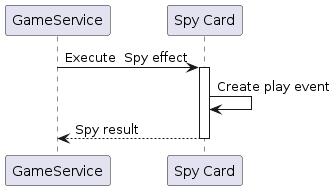
\includegraphics[width=\textwidth]{diagrams/SpyCardPlay.png}
        \caption{Jogada da carta Espião. Fonte: os autores}
        \label{fig:spy-card-play}
    \end{minipage}
    \hfill
    \begin{minipage}{0.48\textwidth}
        \centering
        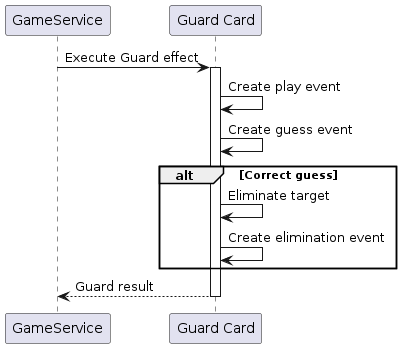
\includegraphics[width=\textwidth]{diagrams/GuardCardPlay.png}
        \caption{Jogada da carta Guarda. Fonte: os autores}
        \label{fig:guard-card-play}
    \end{minipage}
\end{figure}

% Sacerdote (2) e Barão (3)
\begin{figure}[h]
    \centering
    \begin{minipage}{0.48\textwidth}
        \centering
        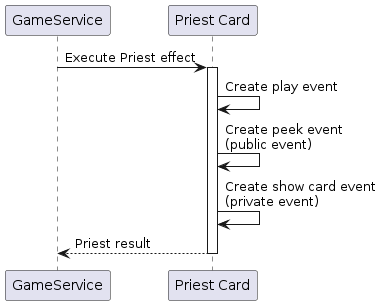
\includegraphics[width=\textwidth]{diagrams/PriestCardPlay.png}
        \caption{Jogada da carta Sacerdote. Fonte: os autores}
        \label{fig:priest-card-play}
    \end{minipage}
    \hfill
    \begin{minipage}{0.48\textwidth}
        \centering
        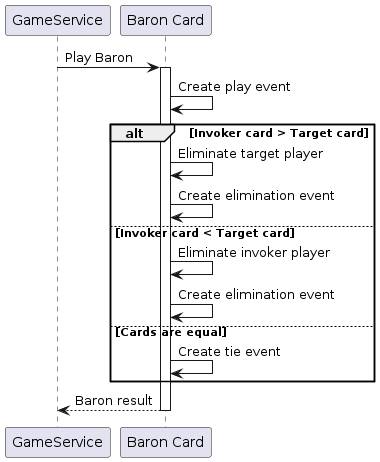
\includegraphics[width=\textwidth]{diagrams/BaronCardPlay.png}
        \caption{Jogada da carta Barão. Fonte: os autores}
        \label{fig:baron-card-play}
    \end{minipage}
\end{figure}

% Criada (4) e Príncipe (5)
\begin{figure}[h]
    \centering
    \begin{minipage}{0.48\textwidth}
        \centering
        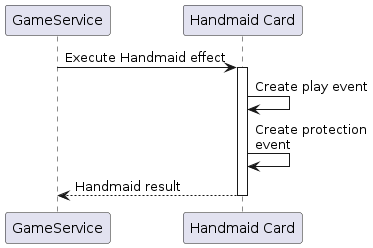
\includegraphics[width=\textwidth]{diagrams/HandmaidCardPlay.png}
        \caption{Jogada da carta Criada. Fonte: os autores}
        \label{fig:handmaid-card-play}
    \end{minipage}
    \hfill
    \begin{minipage}{0.48\textwidth}
        \centering
        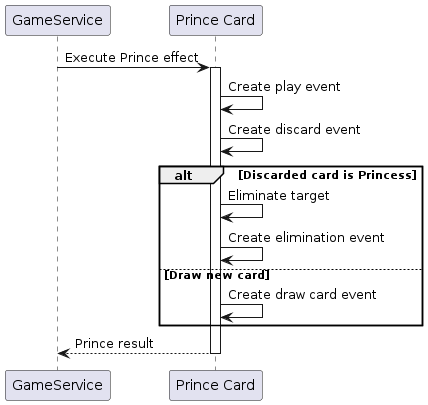
\includegraphics[width=\textwidth]{diagrams/PrinceCardPlay.png}
        \caption{Jogada da carta Príncipe. Fonte: os autores}
        \label{fig:prince-card-play}
    \end{minipage}
\end{figure}

% Chanceler (6) e Rei (7)
\begin{figure}[h]
    \centering
    \begin{minipage}{0.48\textwidth}
        \centering
        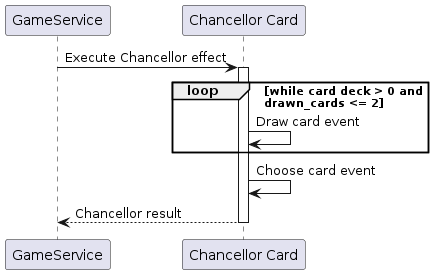
\includegraphics[width=\textwidth]{diagrams/ChancellorCardPlay.png}
        \caption{Jogada da carta Chanceler. Fonte: os autores}
        \label{fig:chancellor-card-play}
    \end{minipage}
    \hfill
    \begin{minipage}{0.48\textwidth}
        \centering
        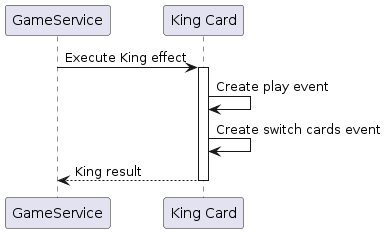
\includegraphics[width=\textwidth]{diagrams/KingCardPlay.png}
        \caption{Jogada da carta Rei. Fonte: os autores}
        \label{fig:king-card-play}
    \end{minipage}
\end{figure}

% Condessa (8) e Princesa (9)
\begin{figure}[h]
    \centering
    \begin{minipage}{0.48\textwidth}
        \centering
        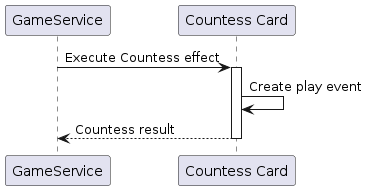
\includegraphics[width=\textwidth]{diagrams/CountessCardPlay.png}
        \caption{Jogada da carta Condessa. Fonte: os autores}
        \label{fig:countess-card-play}
    \end{minipage}
    \hfill
    \begin{minipage}{0.48\textwidth}
        \centering
        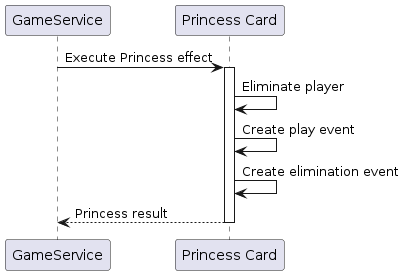
\includegraphics[width=\textwidth]{diagrams/PrincessCardPlay.png}
        \caption{Jogada da carta Princesa. Fonte: os autores}
        \label{fig:princess-card-play}
    \end{minipage}
\end{figure}

\subsection{Estados do Jogo}
O sistema gerencia diferentes estados do jogo para garantir que as ações sejam executadas na ordem correta:

\begin{itemize}
    \item \textbf{WaitingForPlayers}: Aguardando jogadores entrarem na sala
    \item \textbf{WaitingForDraw}: Aguardando o jogador da vez comprar uma carta
    \item \textbf{WaitingForPlay}: Aguardando o jogador escolher e jogar uma carta
    \item \textbf{Finished}: Jogo finalizado
\end{itemize}

\section{Validação de Ações}

O sistema implementa múltiplas camadas de validação para garantir que apenas ações válidas sejam executadas:

\begin{itemize}
    \item \textbf{Validação de Turno}: Apenas o jogador da vez pode executar ações
    \item \textbf{Validação de Estado}: Ações só são permitidas nos estados apropriados do jogo
    \item \textbf{Validação de Cartas}: O jogador deve possuir a carta que deseja jogar
    \item \textbf{Validação de Requisitos}: Cartas com efeitos específicos requerem parâmetros adicionais
\end{itemize}

\section{Experiência do Usuário}

\subsection{Interface Responsiva}
O frontend desenvolvido em Svelte oferece uma interface moderna e responsiva, com animações suaves que podem ser desabilitadas para melhorar a performance em dispositivos menos potentes.

\subsection{Feedback Visual}
O sistema fornece feedback visual claro para todas as ações:

\begin{itemize}
    \item \textbf{Indicadores de Turno}: Mostra claramente de quem é a vez
    \item \textbf{Log de Jogo}: Mantém histórico de todas as ações executadas
    \item \textbf{Animações de Cartas}: Visualiza movimentação e efeitos das cartas
    \item \textbf{Notificações de Estado}: Informa mudanças importantes no jogo
\end{itemize}

\subsection{Acessibilidade}
O sistema inclui recursos de acessibilidade como:

\begin{itemize}
    \item \textbf{Suporte a Múltiplos Idiomas}: Interface disponível em português, inglês e espanhol
    \item \textbf{Controles Intuitivos}: Interface clara e fácil de navegar
\end{itemize}

Esta arquitetura garante que o sistema Love Letter ofereça uma experiência de jogo fluida, segura e envolvente para todos os participantes, mantendo a fidelidade às regras originais do jogo enquanto aproveita as capacidades da tecnologia moderna para criar uma experiência multiplayer online robusta.
